\documentclass[a4paper]{article}

\usepackage[T1]{fontenc}
\usepackage[utf8]{inputenc}
\usepackage[a4paper]{geometry}
%\usepackage[francais]{babel}
%\usepackage{subfigure}
%\usepackage{fancyvrb}
%\usepackage{fancyhdr}
\usepackage[hypertex,ps2pdf]{hyperref}
\usepackage{array}
\usepackage{xcolor}
%\usepackage{comment}
\usepackage{lmodern}
\usepackage{varwidth}
\usepackage{tikz}
%\usetikzlibrary{arrows}
\usetikzlibrary{automata}
\usetikzlibrary{matrix}
\usetikzlibrary{shapes}
\usetikzlibrary{positioning}
\usepackage{macros}

% fontes tt avec gras (mots-cl�s)
\renewcommand{\ttdefault}{txtt}

% Figures tikz

\tikzstyle{hierarchical state} =
  [rectangle,
   round corners,
   draw=black]

\tikzstyle{ls node} =
  [rectangle,
   sharp corners,
   draw=black]

\tikzstyle{file} =
  [rectangle,
   sharp corners,
   draw=black]

\tikzstyle{tool} =
  [rectangle,
   rounded corners,
   draw=black]

\newenvironment{lsnode}[2][]{
    \node[% title
      ls node
%      fill=blue!90!black,
      ] (title) {#2};% title text
    \node at (title.south west) [%
      ls node,
      anchor=north west,
      yshift=\pgflinewidth]
    \bgroup
       \begin{varwidth}{0.9\textwidth}
         \centering
         \begin{tikzpicture}[%
           node distance=8mm,
           pin distance=8mm,
           label distance=2mm,
           inner sep=1mm,
           anchor=center,
           pos=0.5,
           #1]% optional parameter(s)
}{%
         \end{tikzpicture}
       \end{varwidth}
    \egroup;
}

\newenvironment{contlsnode}[2][]{
    \node[% title
      ls node
%      fill=blue!90!black,
      ] (title) {#2};% title text
    \node at (title.south west) [%
      ls node,rectangle split, rectangle split parts=3,
      anchor=north west,text badly ragged,
      yshift=\pgflinewidth]
    \bgroup
%        \begin{varwidth}{0.9\textwidth}
%          \centering
%          \begin{tikzpicture}[%
%            node distance=8mm,
%            pin distance=8mm,
%            label distance=-0.5mm,
%            inner sep=1mm,
%            anchor=center,
%            pos=0.5,
%            #1]% optional parameter(s)
}{%
%          \end{tikzpicture}
%        \end{varwidth}
    \egroup;
}


\pagestyle{empty}

\begin{document}

\begin{tikzpicture}[node distance=3cm,auto,initial text=,initial where=left,pos=0.5]
  \draw node[state,initial,label={above:$y=\False$}] (A) {A};
  \draw node[state,label={below:$y=\True$}] (C) [below of=A] {C};
  \draw node[draw,rounded corners,anchor=west] (B)
  [right of=A,anchor=north west] {
    \begin{varwidth}{\textwidth}
      \begin{tikzpicture}
        \matrix (m) [matrix of nodes] {
          \begin{tikzpicture}
            \begin{scope}[node distance=2cm,auto,initial text=,initial
              where=left,pos=0.5]
              \draw node[state,initial,label={right:$y_1 =\False$}] (Idle) {Idle};
              \draw node[state,label={right:$y_1=\True$}] (Active) [below of=Idle]
              {Act};
              \path[->] (Idle) edge [bend left] node {$c$} (Active)
              (Active) edge [bend left] node {$c$} (Idle);
            \end{scope}
          \end{tikzpicture}
          &
          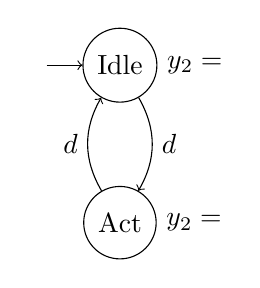
\begin{tikzpicture}
            \begin{scope}[node distance=2cm,auto,initial text=,initial where=left,pos=0.5]
              \draw node[state,initial,label={right:$y_2 =\False$}] (Idle) {Idle};
              \draw node[state,label={right:$y_2=\True$}] (Active) [below of=Idle]
              {Act};
              \path[->] (Idle) edge [bend left] node {$d$} (Active) (Active) edge
              [bend left] node {$d$} (Idle);
            \end{scope}
          \end{tikzpicture}
          \\[5mm]
          \node {$y = y_1\land y_2$};\\
        }; 
        \draw [dashed] (m-1-1.north east) -- (m-1-1.south east);
        \draw [dashed] (m-1-1.south west) -- (m-1-2.south east);
      \end{tikzpicture}
      \end{varwidth}
    };
    \path[->] (A) edge [bend left] node {$c$} (B)
              (B.west) edge [bend left] node {$c\land d$} (C)
              (C) edge [bend left] node {$d$} (A);
  \end{tikzpicture}

\end{document}
